\documentclass[a4paper,11pt]{article}

\usepackage{../../zyancamlec}

\def\ntripos{Mathematical Tripos}
\def\npart{III}
\def\ncourse{Symmetries, Fields and Particles}
\def\nscourse{SFP}
\def\nlecturer{B.\ Allanach}
\def\nterm{Michaelmas}
\def\nyear{2020}

\usepackage{tikz-feynhand}

\begin{document}
	\maketitlepage
	\preliminaries

	\section*{Course Information}

	Lie groups and Lie algebras are important in the construction of quantum field theories which describe interactions between known particles. Gauge theories, which describe many of the interactions in the Standard Model, rely on them. After some other preliminaries, we introduce representations in terms of square matrices. The group of rotations in three-dimensional space SO(3) is covered, along with SU(2) and the connection to angular momentum. Relativistic symmetries are discussed: in particular, the Lorentz and Poincar\'e groups and quantum fields. Lie groups and Lie algebras are covered in more generality, focusing on SU(3) as a useful example. An overview of the results of the Cartan classification of simple Lie algebras is included. Finally, gauge theory is introduced.
	
	\section*{Pre-requisites}

	Linear algebra including direct sums and tensor products of vector spaces. Special relativity and quantum theory, including orbital angular momentum theory and Pauli spin matrices.
  
	\newpage
	\tableofcontents
	\newpage
	\maintext
	\setcounter{section}{-1}
	\section{Introduction}
	\subsection{Symmetries} \lecnr{1}
	\begin{defi}
		A \emph{group} $G$ is a set $G = \{g_1, g_2, \dots\}$ with
		\begin{enumerate}
			\item A composition rule (binary operation) $*$ such that $g * g' \in G, \forall g,g' \in G$, which we shall write as $gg'$;
			\item A unique identity $e$ such that $eg=ge=g, \forall g \in G$;
			\item Associativity: $(gg')g'' = g (g'g'') := gg'g'', \forall g,g',g''\in G$;
			\item A unique inverse $\forall g\in G, \exists g^{-1}$ such that $g g^{-1} = g^{-1} g = e$.
		\end{enumerate}

		If the binary operation is commutative, we say that $G$ is \emph{abelian}.
	\end{defi}

	\begin{ex}
		Group $\mathbb{Z}_n = \{0,1,\dots,n-1\}$ with group operation being addition modulo $n$ and identity $e = 0$.

		Cyclic group $C_n = \{e^{2\pi \mathrm{i} r/n} \in \mathbb{C} : r = 0,1,\dots,n-1\}$, certain complex numbers of modulus 1, under multiplication.

		$\mathbb{Z}_n$ and $C_n$ are clearly abelian. In fact, $C_n \cong \mathbb{Z}_n$, i.e.\ they're \emph{isomorphic}, that is to say there exists a one-to-one correspondence between the elements consistent with group composition rules.
	\end{ex}

	\begin{ex}
		Symmetry groups such as the dihedral group $D_3$ \needfig{1} containing reflections along axes and rotations by $120^\circ, 240^\circ, 360^\circ$. 
	\end{ex}
	
	\begin{ex}
		\emph{Lie groups} are the generalisation to continuous symmetries, e.g.\ rotations by $\theta \in \mathbb{R}$ of a circle (``SO(2)''). Lie groups are essential to the description of particles and their interactions.
	\end{ex}

	To identify the connection between symmetries and groups, we first make the following definition.

	\begin{defi}
		A \emph{symmetry} is a transformation that leaves physical properties (e.g.\ energy, scattering probability, etc.) unchanged. They have properties:
		\begin{itemize}
			\item Symmetries can be composed: $gg' :=$ act first with $g'$, then with $g$;
			\item Doing nothing is a symmetry, $e$, the identity;
			\item A symmetry transformation $g$ can be reversed by $g^{-1}$, which is itself a symmetry.
		\end{itemize}
	\end{defi}

	From above, it is clear that the set of all symmetries forms a group. Symmetry often greatly simplifies analysis. It leads to conservation rules and constrains interactions.

	\subsubsection{Internal Symmetries}

	\emph{Internal symmetries} are properties of particles or fields themselves. 
	\begin{ex}[Colour states of a quark]
		Quarks come in three otherwise identical copies --- called `colours' ({\color{red}red}, {\color{green}green} and {\color{blue}blue}). One can continuously rotate the colours into each other, resulting in a symmetry.

		One can rotate the colour differently at different points of spacetime. In fact, one finds that one has to add a force-carrying particle to make the whole theory invariant under the symmetry. This is the gluon, which carries a colour and an anti-colour. Below is a Feynman diagram representing the fusion of a quark and an anti-quark
		\begin{center}
			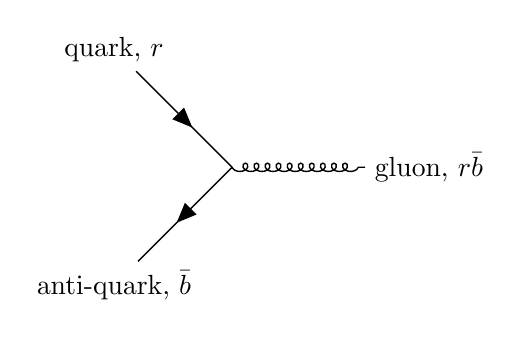
\begin{tikzpicture}
				\begin{feynhand}
					\vertex (aq) at (0,0) {anti-quark, $\bar{b}$};
					\vertex (q) at (0,3) {quark, $r$};
					\vertex [particle] (v) at (1.5,1.5);
					\vertex (f) at (4,1.5) {gluon, $r \bar{b}$};
		
					\propag [fer] (q) to [] (v);
					\propag [antfer] (aq) to [] (v);
					\propag [glu] (v) to [] (f);
				\end{feynhand}
			\end{tikzpicture}
		\end{center}

		Anti-quarks carry anti-colour $\{\bar{r}.\bar{g},\bar{b}\}$. The group structure implies that colour is conserved by interactions (i.e.\ $r \bar{b} \to r \bar{b}$ in $q \bar{q}\to g$).
	\end{ex}
	When the theory is left invariant by a symmetry transformation that's the same across whole spacetime, it's called a \emph{global symmetry}. 

	The theory of quarks, anti-quarks and gluons is called \emph{Quantum Chromodynamics} (QCD), which is a part of the Standard Model of particle physics.

	Since the colour rotations may differ at different points $(\vb x,t)$ in spacetime, it is called a \emph{local} or \emph{gauge} symmetry.

	\subsubsection{External Symmetries}

	\emph{External symmetries} involve spacetime coordinates.

	\begin{ex}
		\ 
		\begin{itemize}
			\item Translation in $(\vb x,t)$;
			\item Lorentz transformation: boosts/rotations;
		\end{itemize}
	\end{ex}

	Conserved quantities come from the group structure: e.g.\ energy, momentum, angular momentum, etc. The \emph{Poincar\'e group} consists of all these symmetries: 3 boosts, 3 rotations and 4 translations.

	Group theory has also been used in cases where the symmetries are approximate but not exact, to explain the spectrum of hadrons, for instance.

	\subsection{Particles}
	\subsubsection{Force-carriers} 
	
	Force-carriers are particles with spin 1($\hbar$) (convention $\hbar \to 1$, see QFT course).
	
	\begin{ex}
		\ 
		\begin{itemize}
			\item $g$, gluon carries colour force;
			\item $\gamma$, photons carry the electromagnetic force.
			\item $W^{\pm}, Z^0$ boson carry electroweak force that mediates radioactive decay.
		\end{itemize}
	\end{ex}

	\begin{nt}
		Bosons are integer spin particles. Fermions are half-integer spin particles.

		For spin 2, we have graviton, the force carrier of gravity. It is not seen yet because gravity is so weak.
	\end{nt}

	Force carriers belonging to a good symmetry are \emph{massless}. Those corresponding to one where the vacuum ``spontaneously'' breaks an underlying symmetry may be massive (i.e.\ $W^\pm, Z^0$ bosons, the symmetry is broken by the Higgs mechanism).

	\subsubsection{Matter Particles} 
	Matter particles are of spin $\frac{1}{2}$.
	\begin{ex}
		\
		\begin{itemize}
			\item Up quarks, electric charge $Q = + 2/3$ (choosing units where $e = 1$);
			\item Down quarks, $Q = -1/3$; 
			\item Neutrinos, $Q = 0$;
			\item Electrons, $Q = -1$.
		\end{itemize}

		They all have anti-particles, with opposite sign charge or anti-colour.
	\end{ex}

	Matter particles additionally come in 3 families, each are heavier than the last but otherwise with the same colour and charge.

	\begin{table}[H]
		\centering
		\begin{tabular}{c|c|c|c|c}		
			\hline
			Family & $Q = + 2/3$ & $Q = - 1/3$ & $Q = -1$ & $Q = 0$ \\
			\hline
			1 & up $u$ & down $d$ & electron $e$ & $e$-neutrino $\nu_e$\\
			2 & charm $c$ & strange $s$ & muon $\mu$ & $\mu$-neutrino $\nu_\mu$\\
			3 & top $t$ & bottom $b$ & tauon $\tau$ & $\tau$-neutrino $\nu_\tau$\\
			\hline
		\end{tabular}		
	\end{table}

	Anti-particles are denoted with a bar above, e.g.\ $\bar{\nu}_e, \bar{u}$, etc.

	The Standard Model explains many of these features with a QFT possessing a particular group structure of symmetries. Each particle has its own field which fills the spacetime. Quantum excitations of the fields are observed in experiments.
\end{document}